\documentclass[conference]{IEEEtran}
\IEEEoverridecommandlockouts
% The preceding line is only needed to identify funding in the first footnote. If that is unneeded, please comment it out.
\usepackage{cite}
\usepackage{amsmath,amssymb,amsfonts}
\usepackage{algorithmic}
\usepackage{graphicx}
\usepackage{subcaption}

\usepackage[linesnumbered,ruled]{algorithm2e}



\usepackage{textcomp}
\usepackage{xcolor}
\def\BibTeX{{\rm B\kern-.05em{\sc i\kern-.025em b}\kern-.08em
    T\kern-.1667em\lower.7ex\hbox{E}\kern-.125emX}}
    
    
\graphicspath{ {./imgs/} }
    
\begin{document}

\title{Orange Detection Algorithm}

\author{\IEEEauthorblockN{Marshall Asch}
\IEEEauthorblockA{\textit{University of Guelph}\\
Guelph, Canada \\
masch@uoguelph.ca}
\and
\IEEEauthorblockN{Grant Douglas}
\IEEEauthorblockA{\textit{University of Guelph}\\
Guelph, Canada \\
gdouglas@uoguelph.ca}
}

\maketitle

\begin{abstract}
This document is a model and instructions for \LaTeX.
This and the IEEEtran.cls file define the components of your paper [title, text, heads, etc.]. *CRITICAL: Do Not Use Symbols, Special Characters, Footnotes, 
or Math in Paper Title or Abstract.
\end{abstract}

\begin{IEEEkeywords}
Image Processing, Fruit, Applied image colour segmentation, Automated counting
\end{IEEEkeywords}

\section{Introduction}

Counting and identifying the number of ripe fruits is important to automate harvesting fruits when they are ripe and to identify how many ripe fruits there are on a tree.

\section{Ease of Use}

\subsection{How we Selected the threshhold vales}


\section{Algorithms}

based off of this \cite{payne_estimation_2013}



\subsection{Values} \label{values}


\begin{figure*}[htbp]
\centerline{\includegraphics[width=\textwidth]{algo_stages}}
\caption{Outline of the proccess of the stages of the algorithm}
\label{fig}
\end{figure*}

\subsection{Stages}



\subsubsection{Step 1}
Run NDI 

\subsubsection{Step 2}
In the RGB colour space run a mean filter.

\subsubsection{Step 3}
convert the image to the YCrCb colour space.

run a threshold on the Cr values. how the threshold is discusses in sec. \ref{values}. 


\subsubsection{Step 4}

run a threshold on the Cb values. how the threshold is discusses in sec. \ref{values}. 

\subsubsection{Step 5}

Then do a bit-wise and to create a mask

\begin{equation}
pixel_{final}=pixel_{NDI} \land pixel_{mean} \land pixel_{Cr} \land pixel_{Cb} 
\end{equation}

\subsubsection{Step 6}
Do a circle count  on the mask image




\section{Results}

\begin{figure*}
  \begin{subfigure}{.33\linewidth}
 	 \includegraphics[width=\linewidth]{citrus1/citrus1_orig.jpg}\hfill
	 \caption{Origonal}
  \end{subfigure}
  \begin{subfigure}{.33\linewidth}
  	\includegraphics[width=\linewidth]{citrus1/citrus1_NDI.jpg}\hfill
   	\caption{Result of step 1}
  \end{subfigure}
  \begin{subfigure}{.33\linewidth}
  	\includegraphics[width=\linewidth]{citrus1/citrus1_mean.jpg}
  	\caption{Result of step 2}
  \end{subfigure}\par\medskip
  
  \begin{subfigure}{.33\linewidth}
  	\includegraphics[width=\linewidth]{citrus1/citrus1_cr.jpg}\hfill
     	\caption{Result of step 3}
  \end{subfigure}
  \begin{subfigure}{.33\linewidth}
  	\includegraphics[width=\linewidth]{citrus1/citrus1_cb.jpg}\hfill
     	\caption{Result of step 4}
  \end{subfigure}
  \begin{subfigure}{.33\linewidth}
  	\includegraphics[width=\linewidth]{citrus1/citrus1_mask.jpg}
  	\caption{Result of step 5}
  \end{subfigure}\par\medskip
  \begin{subfigure}{.5\linewidth}
  	\includegraphics[width=\linewidth]{citrus1/citrus1_circles_mask.png}\hfill
	   	\caption{Result of step 6a}
  \end{subfigure}
  \begin{subfigure}{.5\linewidth}
  	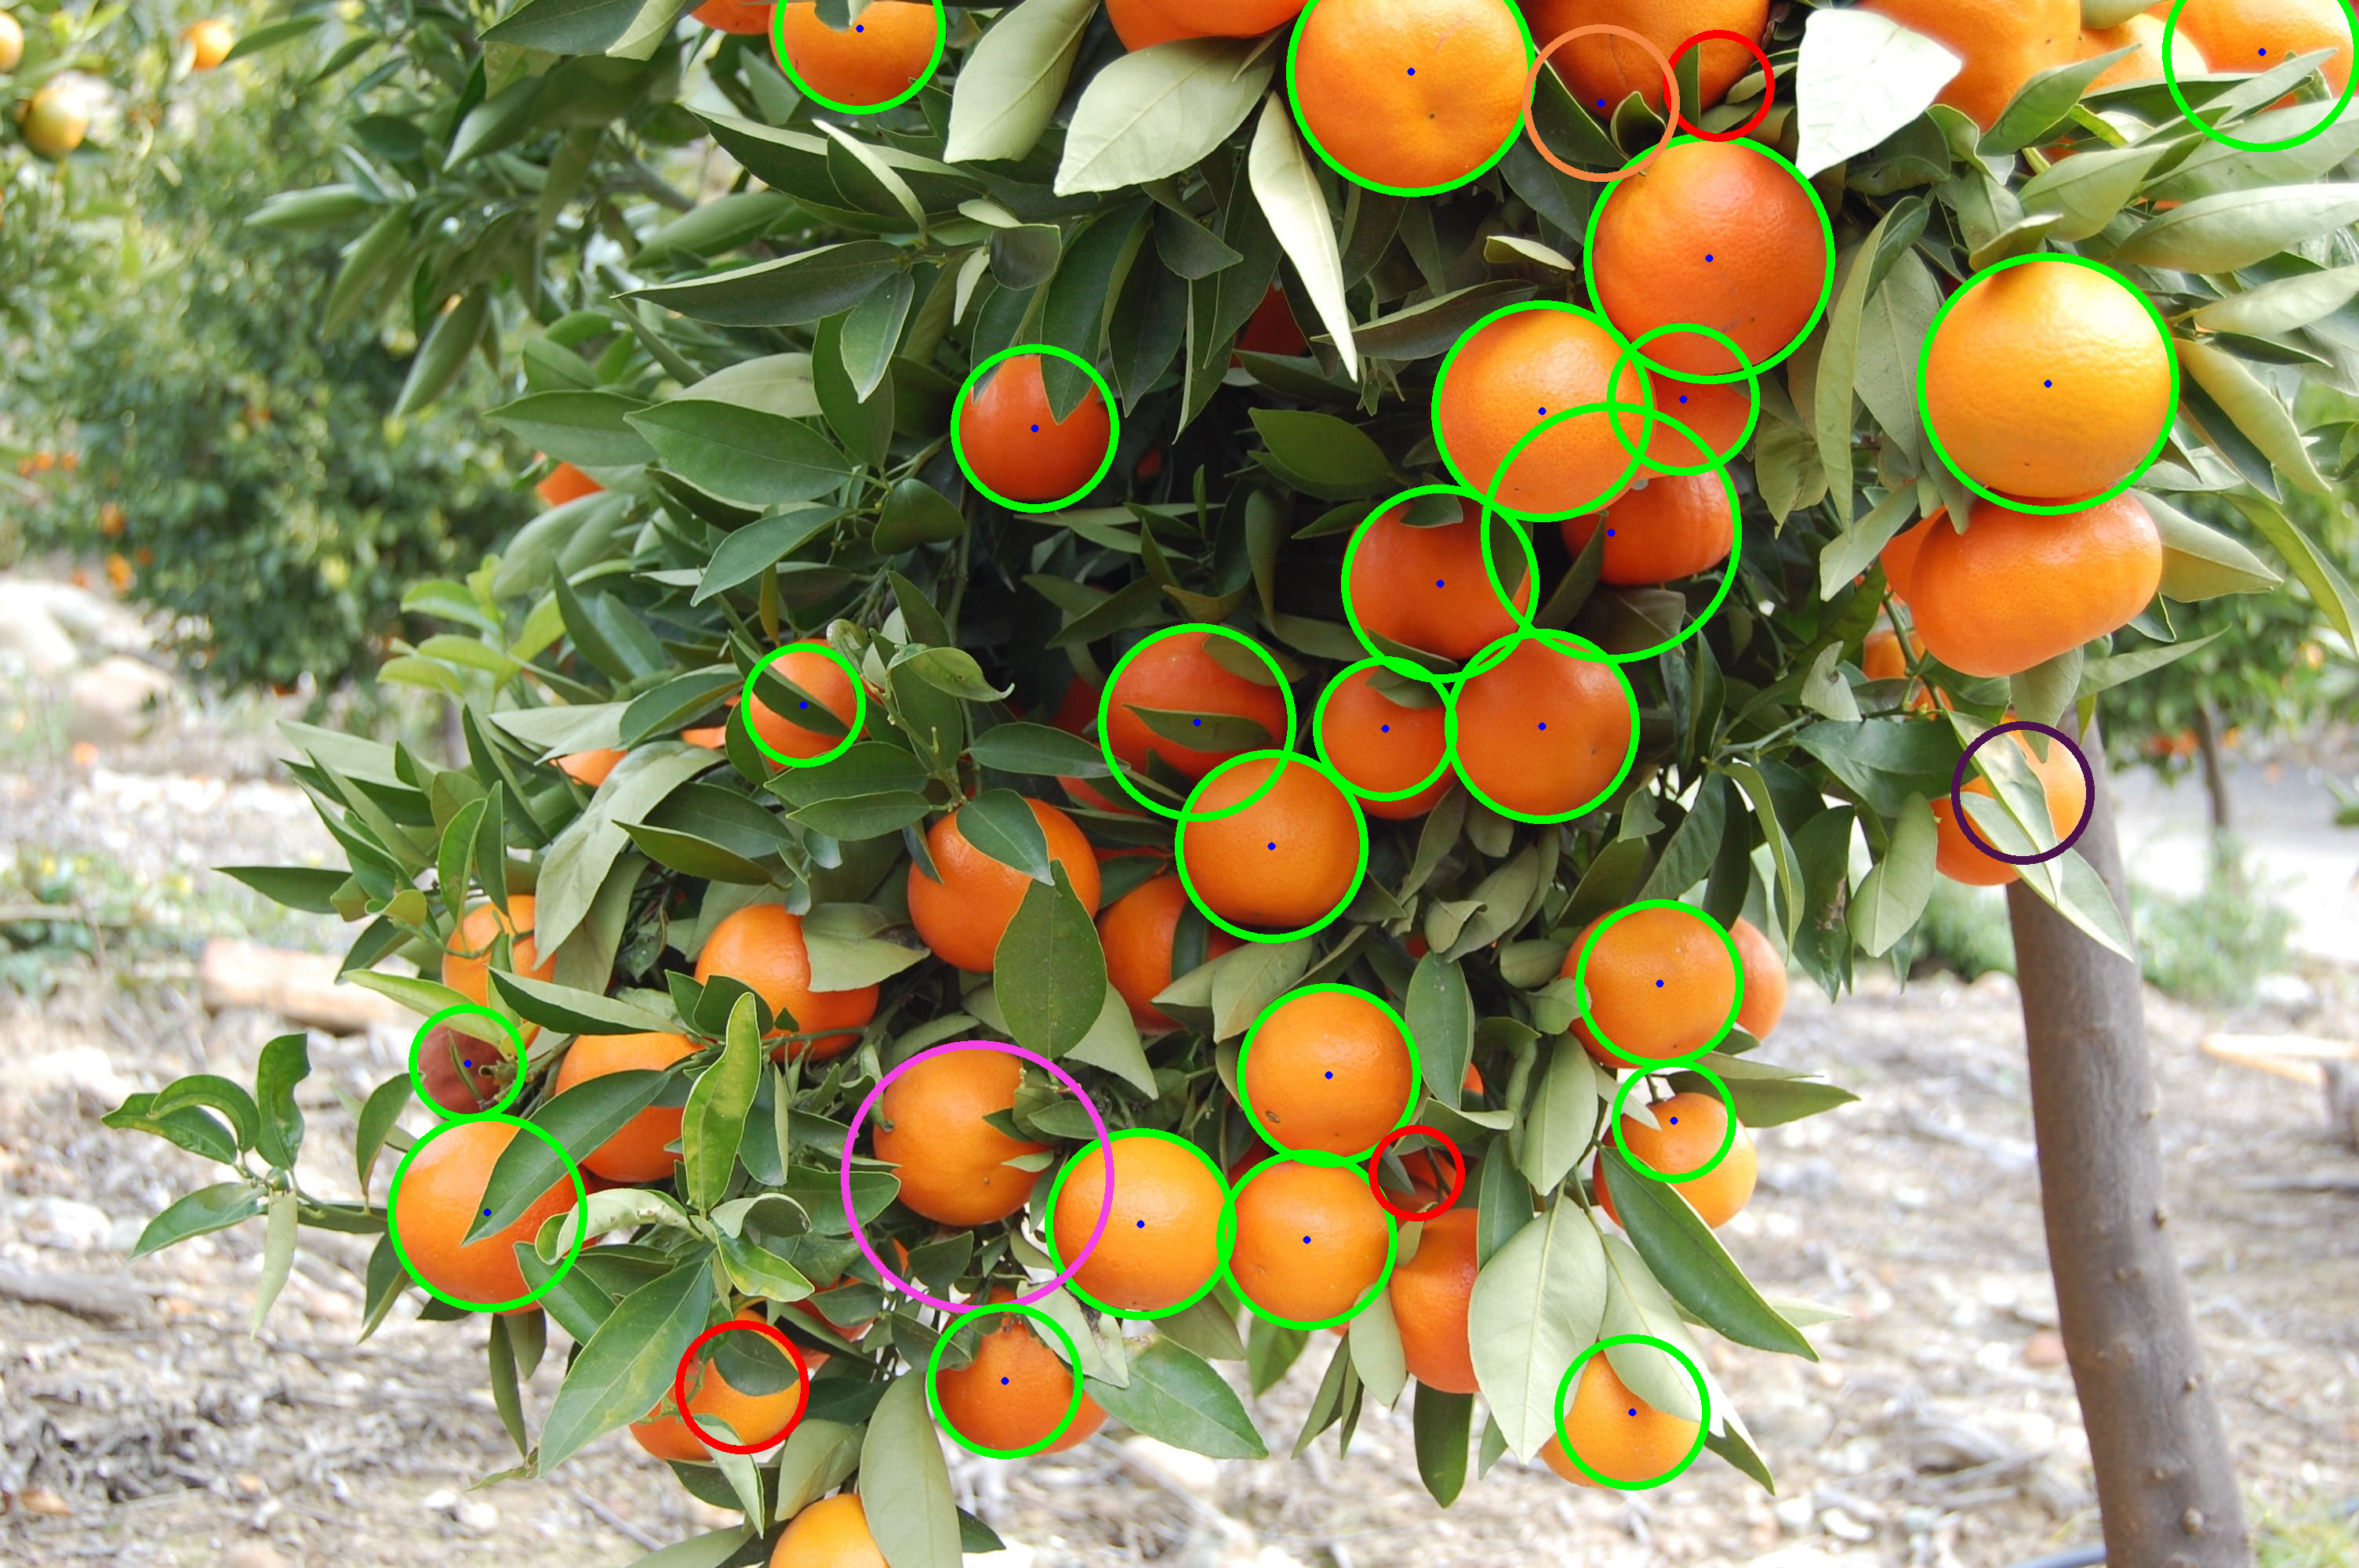
\includegraphics[width=\linewidth]{citrus1/citrus1_circles.png}\hfill
 	 \caption{Result of step 6b}
  \end{subfigure}
  \caption{An example image going through each step to detect the oranges within the image }
\end{figure*}


\section{Discussion}

\subsection{Limitations}

When we were testing our algorithm we noticed that it worked significantly better on images larger than 1300x1300px. It also does not work on images where the diameter of the oranges is greater than half of the screen size, or if the oranges are very small (less then 150px). We determined that this short coming can be easily overcome by using image resolutions above that size. In the application where this algorithm would be used the image quality would be known and the zoom of the image would be consistent allowing the mentioned shortcomings to be overcame. 



\section{Psudo code}

\subsection{Circle Filtering}

\begin{algorithm} 
    \SetKwInOut{Input}{Input}
    \SetKwInOut{Output}{Output}

    \underline{function CountCircles} $(img)$\;
    \Input{Binarized image of the oranges $img$}
    \Output{$NumOranges$}
    
    img = medianBlur(img, 3)
    circles = HoughCircles(img, 2.5, 150, 100, 100, 0, 3000)
    
    found = fillZero(img.size)
    averageR = 0
    
    \For{circle $\in$ circles}{
     ratio = countWhitePixels(img, circle)
     
     notTakenRatio = countNotTaken(found, circle)
     
    \uIf{$circle.radius > img.size/4 \lor ratio <  20$}
      {
        continue
      }
      
      /* make sure that the radius does not differ too much */
      
      \If{$(averageR = 0) \lor (averageR\cdot0.5 \leq circle.radius \leq averageR\cdot1.5$}
      {
      	/* very confident this is an orange*/
	
          \If{$ratio \geq 50$}	
          {
          	averageR = (averageR +  circle.radius) / 2
	
		markFound(found, circle)
		
		markCircle(img, circle, color.GREEN)
	  }
	  \ElseIf{$ratio \geq 30$}{
	  
	  	 \uIf{$averageR\cdot0.8 \leq circle.radius \leq averageR\cdot1.2$}	
          	{
			markCircle(img, circle, color.ORANGE)
	 	 }
	  	\uElseIf{$ circle.radius \leq averageR\cdot1.4$}{
			markCircle(img, circle, color.PURPLE)
	  	}
		\uElse{
			markCircle(img, circle, color.RED)
		}
	  }
	  \Else{
	  	/* not filled enough, but close size*/
		
		\uIf{$averageR\cdot0.8 \leq circle.radius \leq averageR\cdot1.2$} {
			markCircle(img, circle, color.MAROON)
		}
	  }
      }
    }
    \caption{Orange counting algorithms} \label{circleCountAlg}
\end{algorithm}


\begin{algorithm} 
    \SetKwInOut{Input}{Input}
    \SetKwInOut{Output}{Output}

    \underline{function CheckOverlap} $(foundMask, circle, img, whitePixels)$\;
    \Input{mask where the taken regions are set to 1 and untaken set to  0 $foundMask$}
    \Input{the circle that is being checked $circle$}
    \Input{the binarized image of oranges $img$}
    \Input{percentage of pixels that are white $whitePixels$}
    \Output{$if the circle should be ignored$}
    
    \uIf{$whitePixels \leq 50$}
    {
    	return True
    }
        
    circleMask = fillMask(img.size, circle)
    
    areaNotTaken = 0
    
    areaNewOrangeInFrame = 0
    
    areaFilledNotTaken = 0
    
    \For{$i \in img.height$}
    {
    	 \For{$j \in img.width$}
	 {
	 	\lIf{$\neg foundMask[i,j] \land circleMask$}
		{
			areaNotTaken++
		}
		
		\lIf{$circleMask$}
		{
			areaNewOrangeInFrame++
		}
		
		\lIf{$\neg foundMask[i,j] \land circleMask \land img[i,j]$}
		{
			areaFilledNotTaken++
		}
	 }
    }
    
    /* check that orange is distinct */
    
    \lIf{$areaNotTaken / areaNewOrangeInFrame  \cdot 100 < 10$}
     {
	return False
    }
    
    /* check that non overlaping section is partly filled */
    
    \lIf{$areaFilledNotTaken / areaNewOrangeInFrame  \cdot 100 < 10$}
     {
	return False
    }
    
    return True
    
    \caption{Determine if too much of the circle is already taken by another circle} \label{CheckOverlapAlg}
\end{algorithm}



\begin{algorithm} 
    \SetKwInOut{Input}{Input}
    \SetKwInOut{Output}{Output}

    \underline{function OrangeCount} $(circle, img,)$\;
    \Input{the circle that is being checked $circle$}
    \Input{the binarized image of oranges $img$}
    \Output{percentage of pixels that are white $whitePixels$}
    
        
    circleMask = fillMask(img.size, circle)
    
    circleArea = $  \cdot \pi \cdot circle.radius^2$
    
    numOutOfFrame = circleArea
   
    numOrange = 0
    
    
    \For{$i \in img.height$}
    {
    	 \For{$j \in img.width$}
	 {
	 	numOutOfFrame--
		
	 	\lIf{$img[i,j] \land circleMask$}
		{
			numOrange++
		}
	 }
    }
    
    /* check that enough is in frame*/
    
    \lIf{$numOutOfFrame / circleArea  \cdot 100 > 40$}
     {
	numOrange += numOutOfFrame
    }
    
    percentFilledInFrame = numOrange / numTotal * 100
    
    percentFilled = numOrange / (numTotal - numOutOfFrame) * 100
    
    return min(percentFilledInFrame, percentFilled)
    
    
    \caption{Count the number of pixels that are within the circle that have been marked as orange} \label{OrangeCountAlg}
\end{algorithm}

The accumulator resolution was set to 2.5, experimentation showed this was the best value on out test image set. 
the minimum distance between circles was set to 150px.
the canny edge detection parameters were both set to 100, inorder to use a single threshold, An arbitrary value was chosen between 0 and 255 because the image has been binarized to black in white in an earlier step.
The minimum radious was set to 0 to allow small circles to still be detected, the max was set to 3000 so that all circle will be captured then filtered out lalter. Through experimentation we discovered that if we set the max radius to a smaller value (even tho all the actual circles in the tested images had a radius less than  500px) then valid circles would be missed.


On line 5 in algorithm \ref{circleCountAlg}, the percentage of pixels in the image that have been identified as part of the orange is taken to the number of pixels within the circle that are not part of the orange. Details of this are shown in algorithm \ref{OrangeCountAlg}. The White count algorithm takes into account part of the detected circle that is outside of the frame of the image, if less than 40\% if the circle is outside the frame then that portion that is outside is assumed to be filled, if more then 40\% is outside then it is assumed to not be filled. 


on line 6 of algorithm \ref{circleCountAlg}, the percentage of pixels that are not already taken is counted as part of another orange. This reduces the number of overlapping circles that are detected. This can be seen in figure \ref{overlapComp} where the image on the right does not filter the circles by how much they overlap and the one one on the right does. Details of this are shown in algorithm \ref{CheckOverlapAlg}




\begin{figure}
  \begin{subfigure}{.49\linewidth}
 	 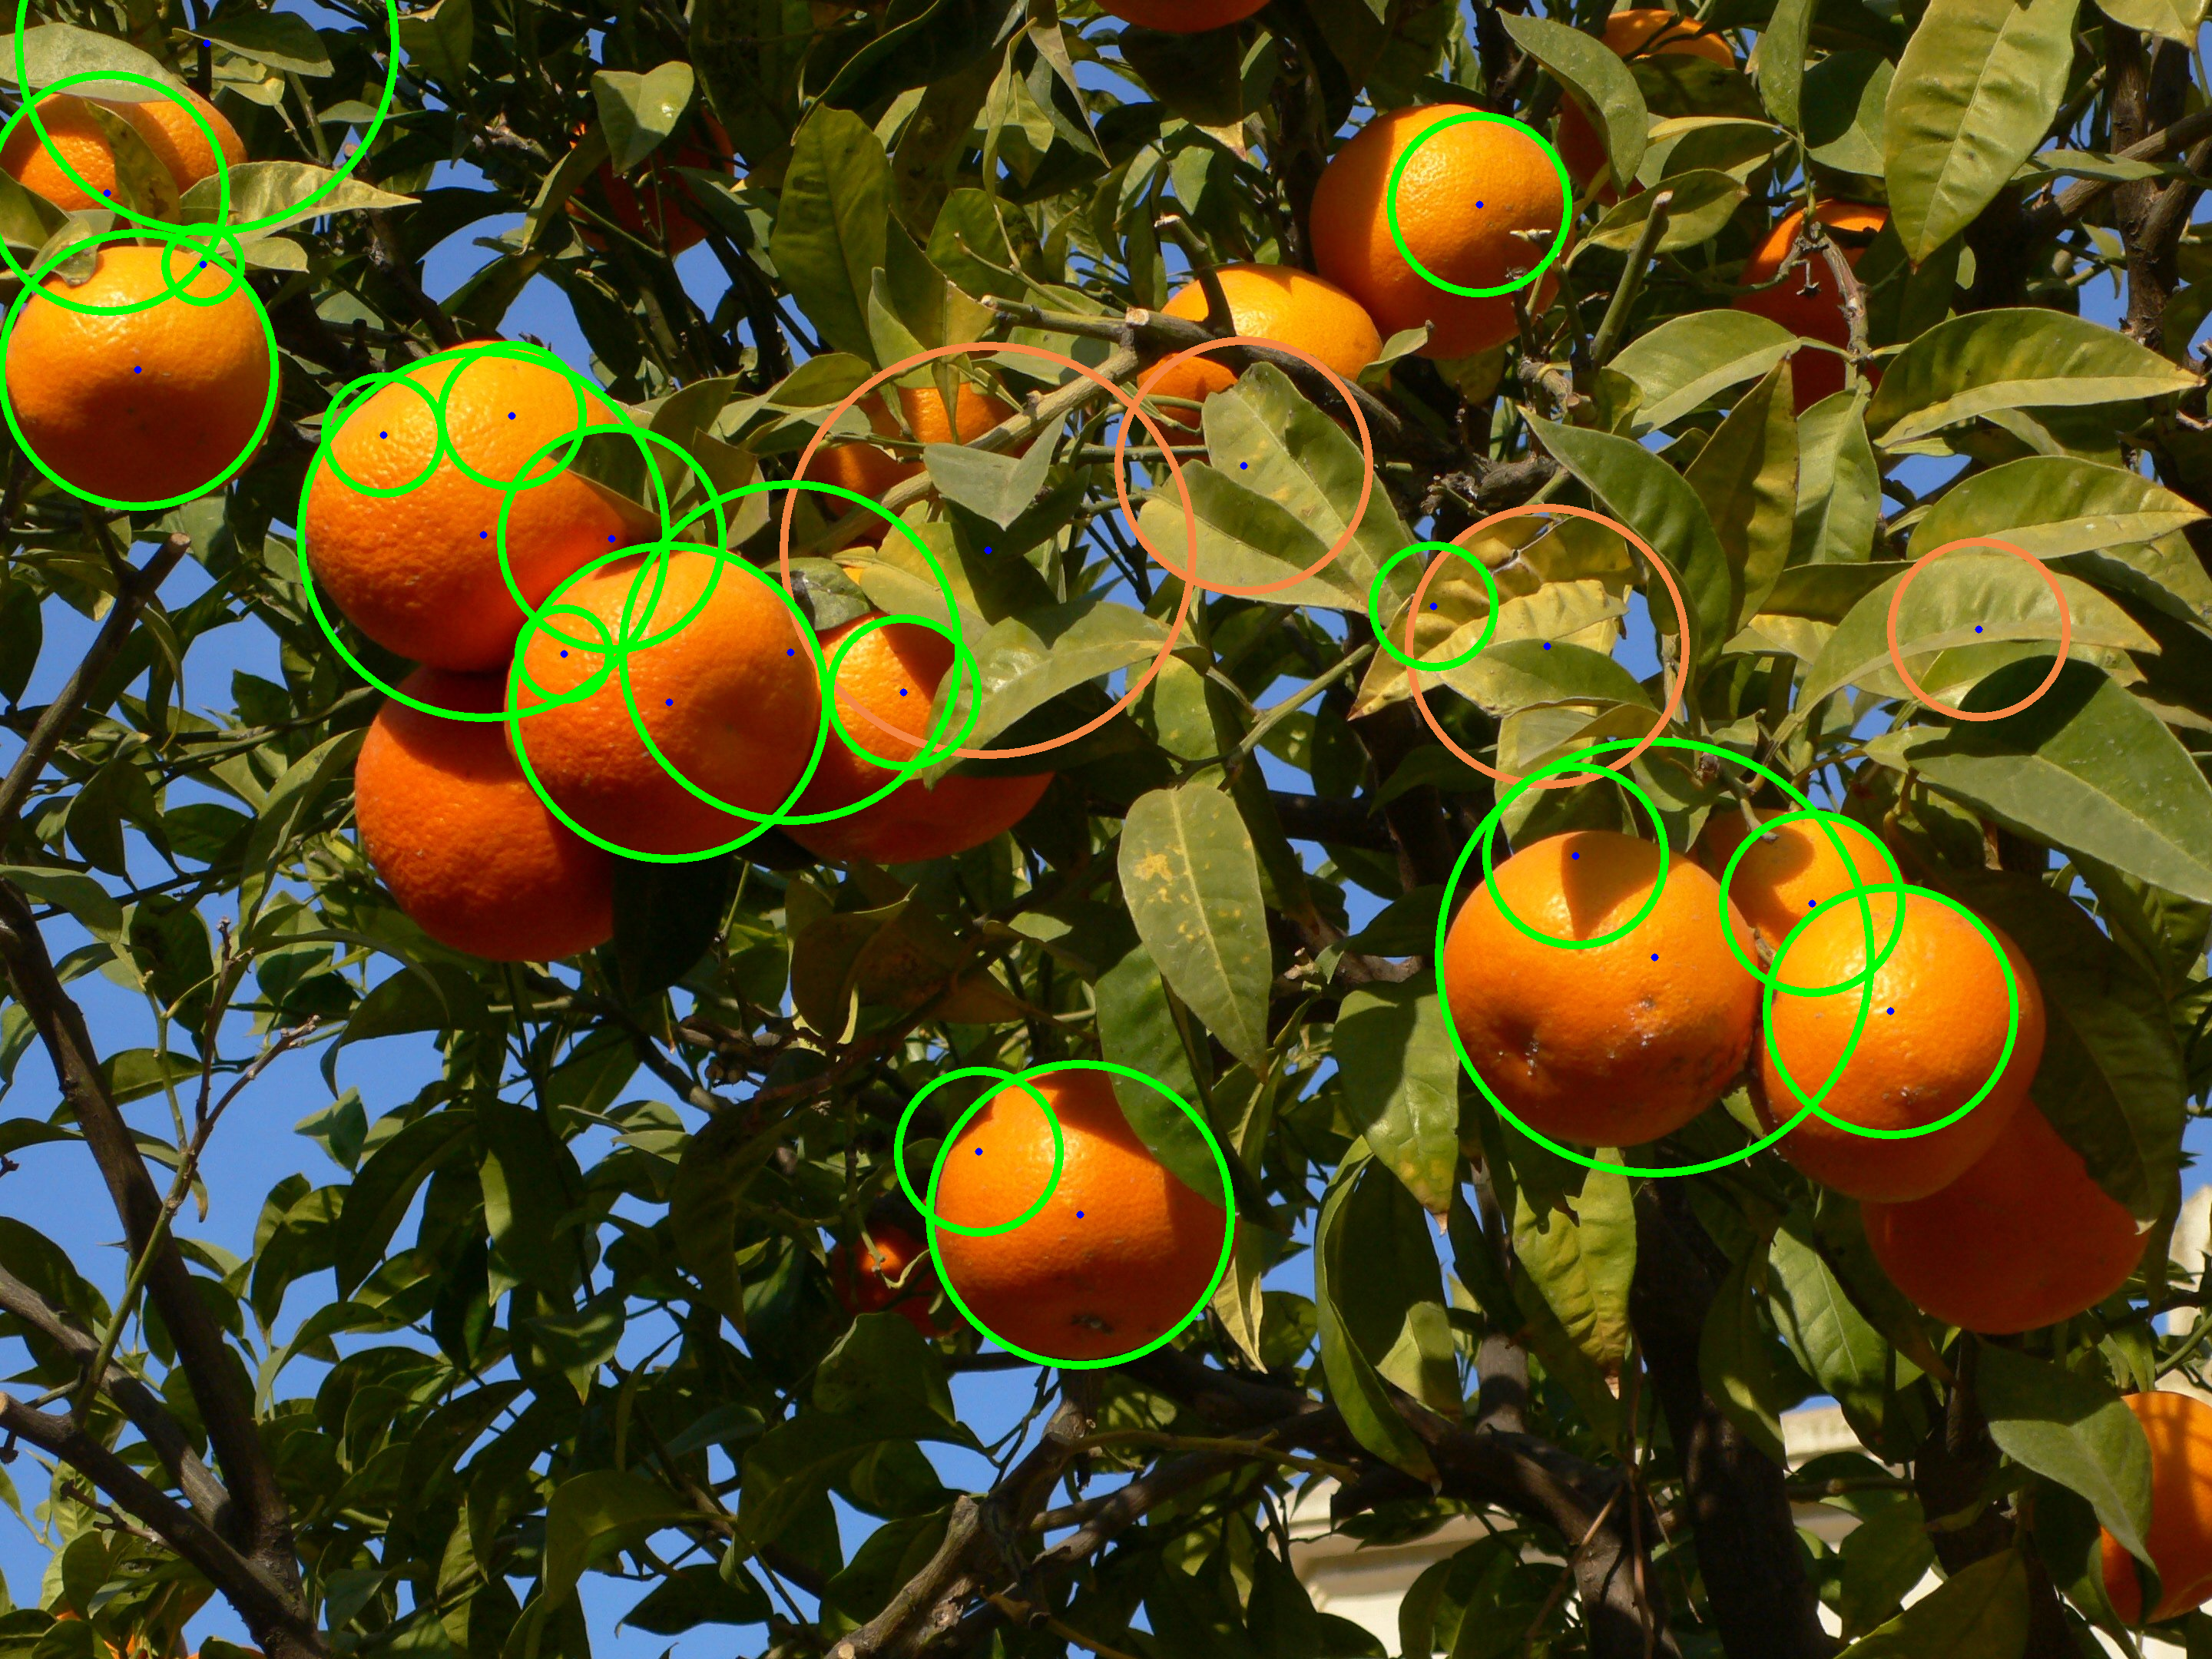
\includegraphics[width=\linewidth]{citrus2_circles.png}\hfill
	 \caption{Filtered out overlapping circles}
  \end{subfigure}
  \begin{subfigure}{.49\linewidth}
  	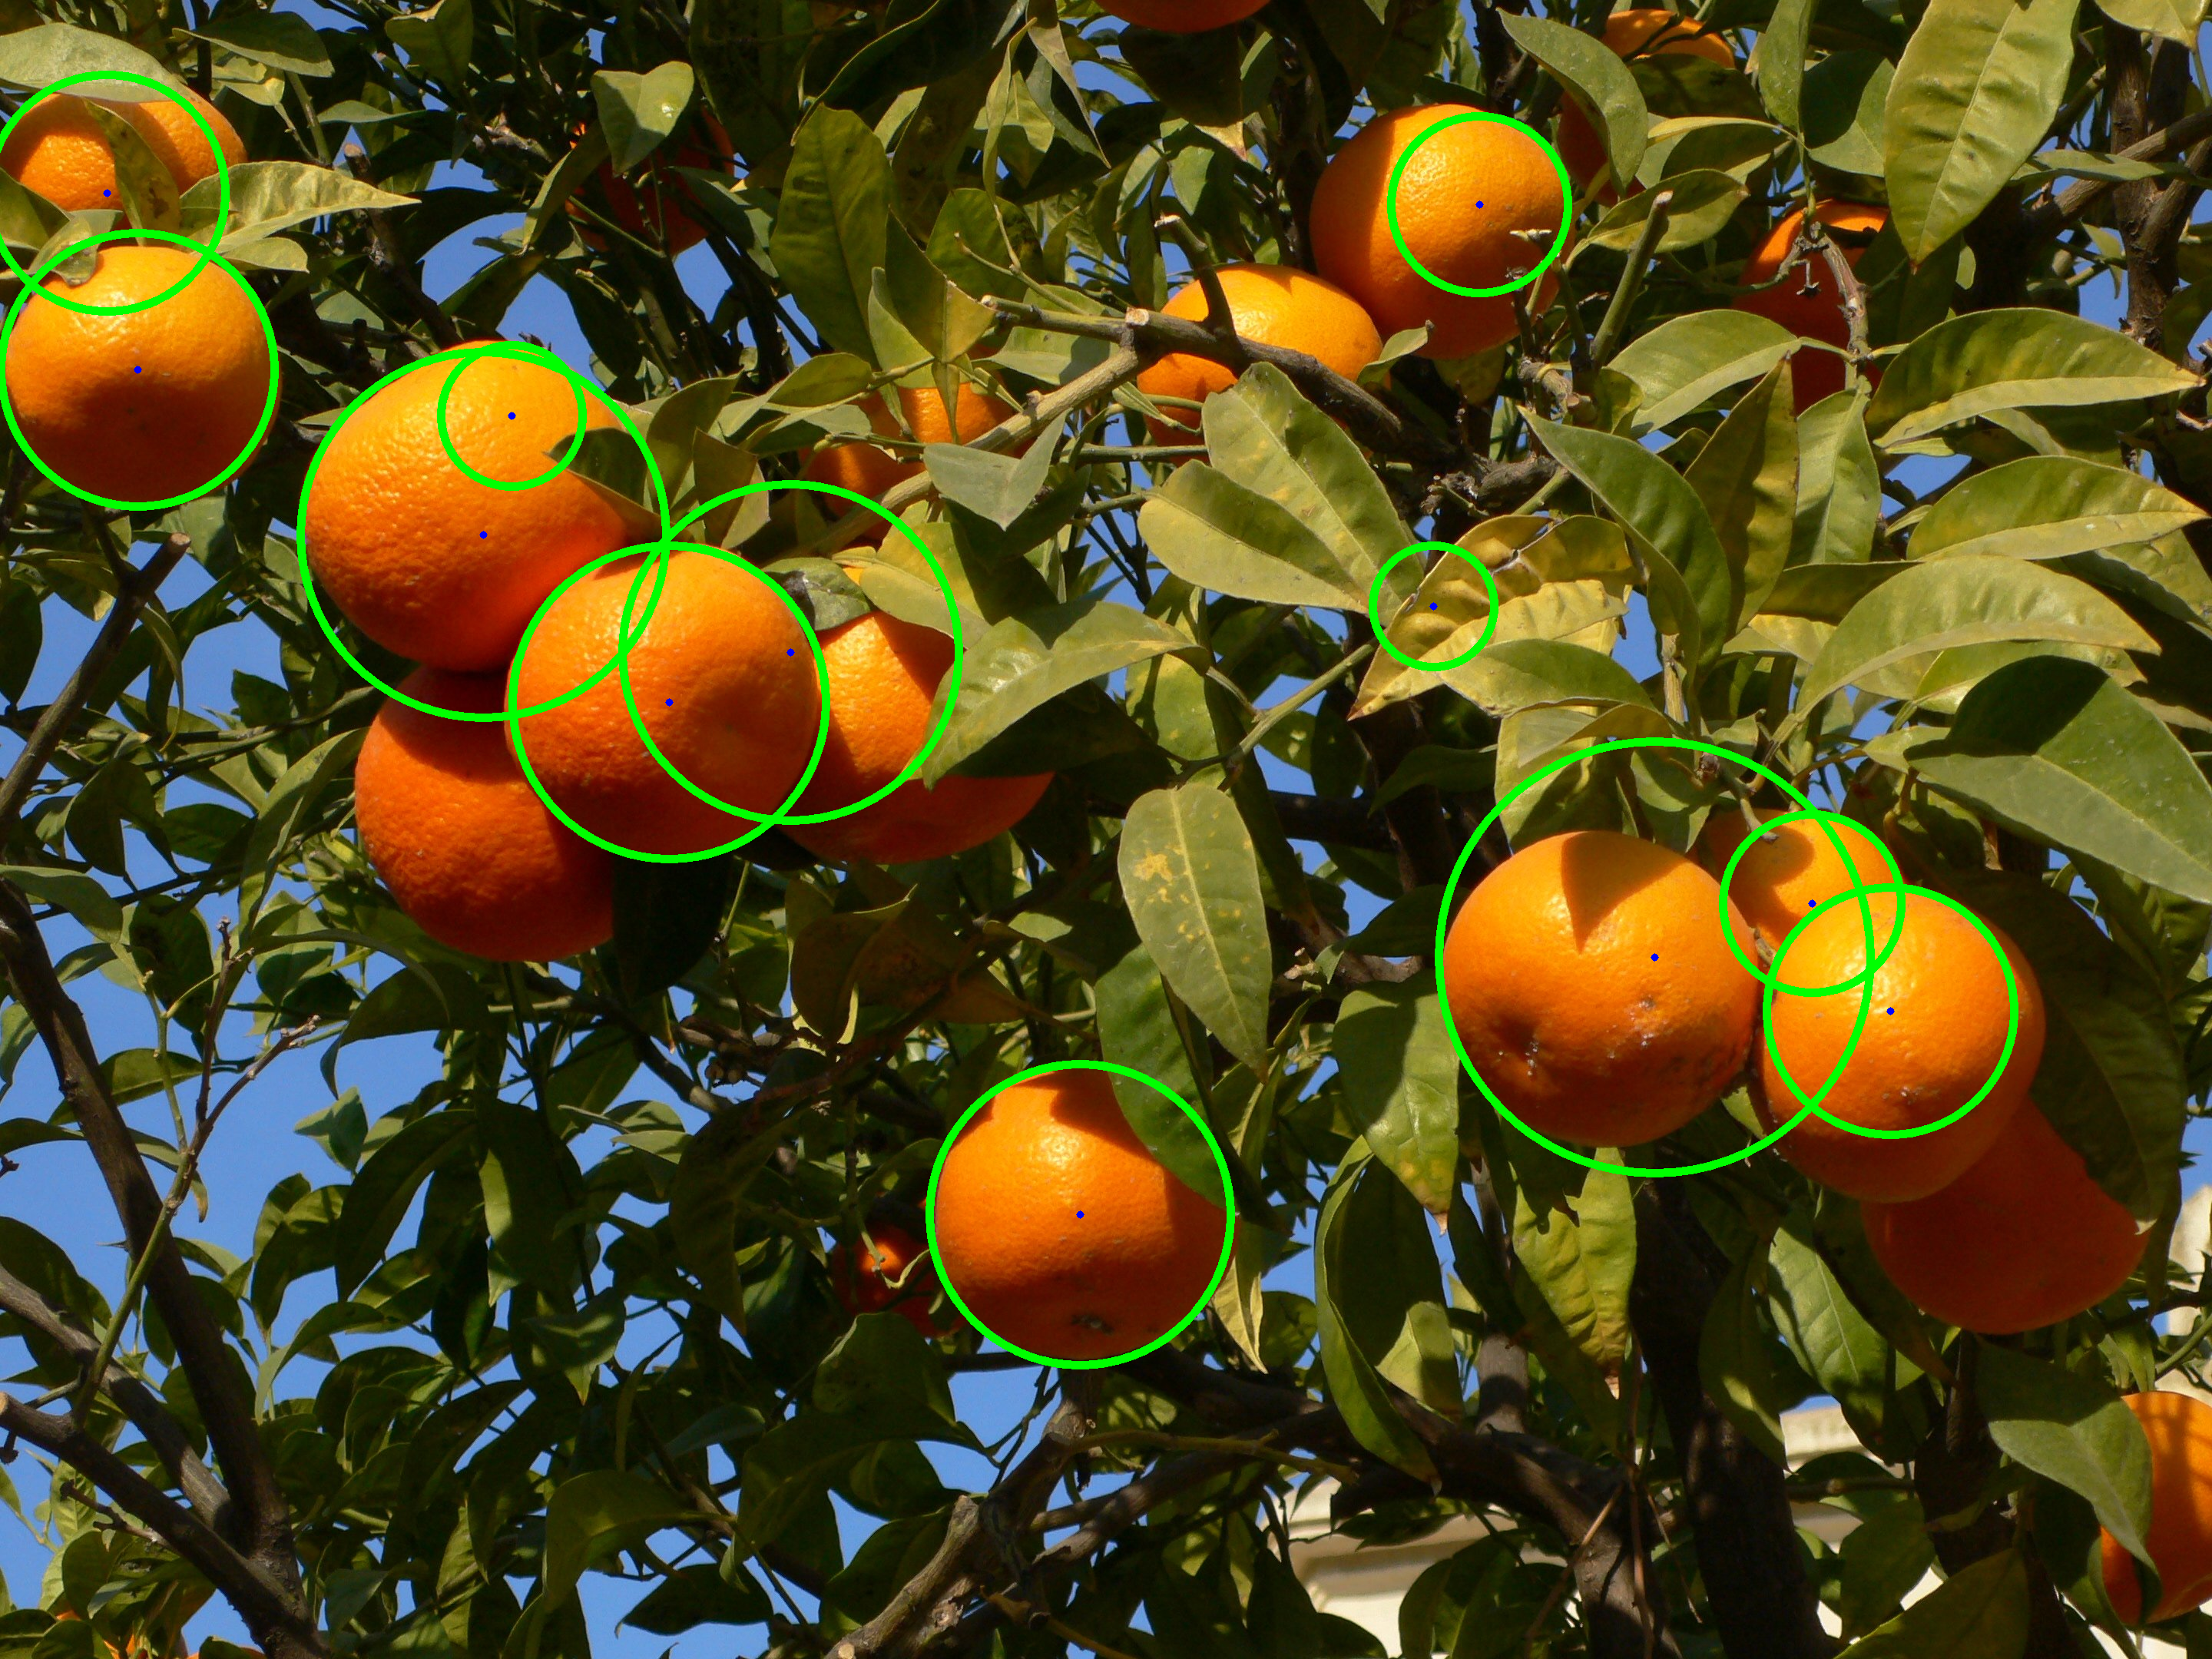
\includegraphics[width=\linewidth]{citrus2_circles_withoverlapfilter.png}
   	\caption{Oranges with overlapping circles}
  \end{subfigure}
  \caption{An example image going through each step to detect the oranges within the image} \label{overlapComp}
\end{figure}




\bibliographystyle{ieeetr}
\bibliography{reference}





\vspace{12pt}

\end{document}
